\documentclass{report}
\usepackage{amsmath}  % Pour les équations mathématiques
\usepackage{graphicx} % Pour insérer des images
\usepackage{geometry} % Pour ajuster les marges
\usepackage{xcolor}  % Pour ajouter des couleurs
\usepackage{amssymb}   % Symboles mathématiques
\usepackage[T1]{fontenc}
\usepackage{siunitx} 
\usepackage{array}      % Tableaux avancés
\usepackage{booktabs} 
\usepackage{multirow}
\geometry{a4paper, margin=1in}


% Définir des couleurs personnalisées
\definecolor{bleu}{RGB}{0, 0, 255}
\definecolor{jaune}{RGB}{255, 255, 0}
\begin{document}

% Page de garde centrée
\begin{center}
    % Logo de l'établissement
    \begin{figure}[h!]
        \centering
        \includegraphics[width=0.5\textwidth]{2725bffcb.JPG} % Remplacez par le chemin de votre logo
        \label{fig:logo}
    \end{figure}

    % Informations sur l'université
     \textbf{\textcolor{bleu}{université sultan moulay slimane}} \\
    \textbf{\textcolor{bleu}{Faculté des Sciences et Techniques - Beni Mellal}} \\
    \textbf{\textcolor{bleu}{Département de génie mécanique}} \\
    \textbf{\textcolor{bleu}{Cycle d'ingénieur en Productique et Mécatronique}} \\

    % Titre du rapport
    \vspace{2cm}
    \LARGE
    \textbf{Rapport de Projet : Robot Auto-Équilibrant} \\
    \vspace{0.9cm}
    \normalsize

    % Image du robot
    \begin{figure}[h!]
        \centering
        \includegraphics[width=0.6\textwidth]{sbf.PNG} % Remplacez par le chemin de votre image du robot
      
    \end{figure}

    % Auteurs et encadrant
    \begin{tabular}{l l}
        \textbf{Réalisé par :} & Ahmed Lablighi \\
                               & Mohamed Ghbal \\
                               & Abdelilah El Hadaoui \\
        \textbf{Encadré par :} & Dr. Zakaria Khaouch \\
    \end{tabular}

    \vspace{1cm}
\end{center}

% Table des matières
\tableofcontents
\vspace{15cm}

% Introduction (non centrée)
\section*{Introduction}

Le concept d’un \textbf{robot auto-équilibrant} repose sur la capacité du robot à maintenir son équilibre de manière dynamique sur deux roues ou une plateforme mobile. Contrairement aux robots traditionnels, qui s’appuient sur une base large et un centre de masse bas pour rester stables, un robot auto-équilibrant doit constamment ajuster sa position pour compenser les perturbations et maintenir une posture verticale. Cette approche permet une mobilité agile et une stabilité dynamique, similaire à celle d’un humain en mouvement.

Ce projet vise à concevoir et à construire un \textbf{robot auto-équilibrant}, capable de se déplacer tout en maintenant son équilibre. Le développement de ce robot englobe plusieurs étapes clés, notamment :
\begin{itemize}
    \item La modélisation des équations de mouvement pour comprendre la dynamique du système.
    \item La conception mécanique et électronique du robot.
    \item La mise en œuvre d’un système de contrôle (comme un régulateur PID) pour assurer l’équilibre dynamique.
    \item La programmation et les tests pour valider les performances du robot.
\end{itemize}

Ce projet représente un défi technique passionnant, combinant des compétences en modélisation physique, conception mécanique, contrôle automatique et programmation. Il offre également une opportunité unique d’explorer des concepts avancés en robotique et en mécatronique, tout en contribuant à l’avancement des connaissances dans ce domaine.

% Motivation (non centrée)
\section*{Motivation}

Les robots traditionnels à plusieurs roues présentent des limitations importantes en termes de stabilité. Un léger décalage du centre de gravité peut rendre le robot instable, et la solution classique consiste à abaisser ce centre de gravité en ajoutant du poids au système. Cependant, cette approche augmente la masse du robot et limite sa vitesse de déplacement, car une vitesse élevée pourrait provoquer son renversement.

Un autre défi des robots traditionnels est leur incapacité à changer de direction de manière agile. Ces robots doivent souvent pivoter pour modifier leur trajectoire, ce qui peut s’avérer difficile, voire impossible, dans des environnements encombrés ou restreints. Cela peut entraîner un blocage du robot et limiter son utilité pratique.

Pour surmonter ces limitations, ce projet explore la \textbf{stabilité dynamique}, une approche qui utilise des algorithmes de contrôle pour maintenir l’équilibre du robot sans dépendre de la stabilité statique. Un exemple bien connu de stabilité dynamique est le \textbf{Segway} (voir Figure \ref{fig:segway}), un véhicule électrique à deux roues alignées axialement. Le Segway utilise la théorie du \textbf{pendule inversé} pour maintenir son équilibre dans la direction longitudinale, tout en reposant sur la stabilité statique dans la direction transversale.

\begin{figure}[h!]
    \centering
    \includegraphics[width=0.5\textwidth]{segway.jpeg} % Remplacez "segway.jpeg" par le nom de votre fichier image
    \caption{Segway, un exemple de robot auto-équilibrant utilisant la stabilité dynamique.}
    \label{fig:segway}
\end{figure}
\vspace{4cm}
Cependant, le Segway présente encore des limitations, notamment sa dépendance à la stabilité statique dans certaines directions. Ce projet vise à aller plus loin en développant un robot \textbf{dynamiquement stable dans toutes les directions}, en s’inspirant des principes du \textbf{Ballbot}. Un Ballbot est un robot qui repose sur une balle sphérique, ce qui lui permet de se déplacer dans n’importe quelle direction tout en maintenant son équilibre de manière dynamique.

Le défi principal de ce projet réside dans la commande d’un système \textbf{sous-actionné}. Un système sous-actionné possède moins d’actionneurs que de degrés de liberté, ce qui signifie que les mêmes actionneurs doivent contrôler plusieurs mouvements simultanément. Par exemple, le Ballbot doit contrôler la position de la balle (dans les directions \(x\) et \(y\)) ainsi que la rotation du corps, ce qui représente un total de 5 degrés de liberté, tout en utilisant seulement 2 à 3 actionneurs.

Ce projet représente une application passionnante de la théorie de commande et de la robotique, avec des implications potentielles pour des domaines tels que la mobilité personnelle, la logistique et l’assistance aux personnes à mobilité réduite.

% Structure du Rapport (non centrée)
\section*{Structure du Rapport}

Ce rapport est organisé de manière à présenter toutes les étapes nécessaires à la réalisation du robot auto-équilibrant, depuis la conception initiale jusqu’aux tests finaux. Chaque section aborde un aspect spécifique du projet, permettant une compréhension claire et progressive du travail accompli.

\subsection*{Chapitre 1 : Introduction}
\begin{itemize}
    \item Présentation du contexte et de la motivation derrière le projet.
    \item Définition des objectifs principaux et secondaires.
    \item Description de la structure globale du rapport.
\end{itemize}

\subsection*{Chapitre 2 : Étude de concept}
\begin{itemize}
    \item Principe fondamental de l'équilibre.
    \item Modèle du pendule inversé.
    \item Étude des technologies et solutions existantes.
\end{itemize}

\subsection*{Chapitre 3 : Conception et implémentation}
\begin{itemize}
    \item Introduction.
    \item Conception mécanique.
    \item Modèle électronique.
\end{itemize}

\subsection*{Chapitre 4 : Simulation}
\begin{itemize}
    \item Implémentation du modèle physique dans MATLAB/Simulink.
    \item Simulation avec LabVIEW pour valider le modèle et le contrôleur PID.
    \item Validation et optimisation des algorithmes de contrôle (PID, etc.).
    \item Analyse des performances théoriques du robot via les résultats de simulation.
\end{itemize}

\subsection*{Chapitre 5 : Fabrication et assemblage}
\begin{itemize}
    \item Liste des matériaux et composants utilisés.
    \item Schémas électroniques et montage des circuits.
    \item Programmation de l’Arduino pour le contrôle du système.
    \item Documentation du processus d’assemblage mécanique et électronique.
\end{itemize}

\subsection*{Chapitre 6 : Conclusion et perspectives}
\begin{itemize}
    \item Synthèse des réalisations et objectifs atteints.
    \item Analyse critique des limitations du projet.
    \item Suggestions pour des améliorations futures ou des extensions possibles 
\end{itemize}

\subsection*{Annexes}
\begin{itemize}
    \item Codes source Arduino et scripts MATLAB.
    \item Plans et dessins techniques issus de SolidWorks.
    \item Fiches techniques des composants utilisés.
    \item Résultats supplémentaires ou données complémentaires.
\end{itemize}



% Suite du document (non centrée)
\chapter{Historique des Robots Auto-Équilibrants}



Ce chapitre traite des \textbf{robots auto-équilibrants}, une catégorie de robots mobiles capables de maintenir leur équilibre de manière dynamique. Ces robots sont souvent conçus pour se déplacer sur une surface tout en compensant les perturbations externes, ce qui les rend particulièrement adaptés à des environnements complexes et changeants. Ce chapitre commence par un aperçu des robots auto-équilibrants les plus connus, suivi d'une discussion sur leur modélisation mathématique et les méthodes de contrôle utilisées pour assurer leur stabilité.

\section{ Aperçu des Robots Auto-Équilibrants Connus}

Plusieurs robots auto-équilibrants ont marqué l'histoire de la robotique, chacun avec des caractéristiques et des applications spécifiques. Voici quelques exemples notables :


\begin{figure}[h]
    \centering
    \includegraphics[width=0.4\textwidth]{R1} % Remplacez R1 par le nom de votre image
    \caption{Segway, un exemple emblématique de système auto-équilibrant.}
\end{figure}


\begin{figure}[h]
    \centering
    \includegraphics[width=0.4\textwidth]{R2} % Remplacez R2 par le nom de votre image
    \caption{NXTway-GS, un robot éducatif à deux roues.}
\end{figure}


\begin{figure}[h]
    \centering
    \includegraphics[width=0.4\textwidth]{R3} % Remplacez R3 par le nom de votre image
    \caption{Balancing Cube, une structure cubique auto-équilibrante.}
\end{figure}
\vspace{12cm}

\section{Modélisation d’un robot auto-équilibrant}

La modélisation d'un robot auto-équilibrant est essentielle pour comprendre son comportement dynamique et concevoir des algorithmes de contrôle efficaces. Ces robots sont souvent modélisés comme des systèmes de type \textbf{pendule inversé}, où l'équilibre est maintenu en ajustant continuellement la position du centre de masse.

\begin{figure}[h]
    \centering
    \includegraphics[width=0.5\textwidth]{R5} % Remplacez R5 par le nom de votre image
    \caption{Modélisation d'un robot auto-équilibrant.}
\end{figure}

\subsection*{Dynamique du système}
Les robots auto-équilibrants sont des systèmes non linéaires et sous-actionnés. Les équations dynamiques décrivent les forces et les moments agissant sur le robot, y compris la gravité, la friction, et les forces générées par les actionneurs (moteurs).

\subsection*{Modèle cinématique}
La cinématique du robot décrit la relation entre les mouvements des roues (ou d'autres éléments de propulsion) et le mouvement global du robot. Cela inclut la vitesse de translation et de rotation.

\subsection*{Modèle de contrôle}
Le contrôle d'un robot auto-équilibrant repose souvent sur des techniques de contrôle optimal, telles que le contrôle par rétroaction linéaire quadratique (LQR) ou le contrôle prédictif (MPC). Ces méthodes permettent de stabiliser le robot tout en minimisant l'énergie consommée.
\vspace{15cm}
\section{ Méthodes de Commande}

Le contrôle d'un robot auto-équilibrant est un défi en raison de sa nature instable. Plusieurs approches ont été développées pour maintenir l'équilibre et permettre une mobilité fluide :

\begin{figure}[h]
    \centering
    \includegraphics[width=1\textwidth]{R6} % Remplacez R6 par le nom de votre image
    \caption{Méthodes de contrôle pour les robots auto-équilibrants.}
\end{figure}
\vspace{10cm}
\subsection*{Contrôle PID}
Un contrôleur proportionnel-intégral-dérivé (PID) est souvent utilisé pour stabiliser le robot en ajustant les forces appliquées en fonction de l'erreur de position et de vitesse. C'est une méthode simple mais efficace pour les systèmes à faible complexité.

\subsection*{Contrôle par rétroaction d'état}
Cette méthode utilise un modèle d'état du système pour calculer les commandes nécessaires pour maintenir l'équilibre. Elle est souvent combinée avec des techniques d'estimation d'état, comme le filtre de Kalman, pour tenir compte des incertitudes du système.

\subsection*{Apprentissage par renforcement}
Des techniques d'apprentissage automatique, comme l'apprentissage par renforcement, ont été explorées pour permettre au robot d'apprendre à maintenir son équilibre de manière autonome. Ces méthodes sont particulièrement utiles dans des environnements imprévisibles.

\section*{ Conclusion}

Les robots auto-équilibrants représentent une avancée majeure dans le domaine de la robotique mobile, offrant une mobilité agile et une capacité à s'adapter à des environnements dynamiques. Leur modélisation et leur contrôle nécessitent une compréhension approfondie de la dynamique des systèmes non linéaires, mais les progrès récents en matière de contrôle optimal et d'apprentissage automatique ouvrent de nouvelles perspectives pour ces robots. Dans les chapitres suivants, nous explorerons plus en détail les aspects techniques et les applications potentielles des robots auto-équilibrants.

\chapter{Étude de concept}

\section{Principe fondamental de l'équilibre}

Un robot auto-équilibrant est un système dynamique qui utilise des moteurs pour compenser l'inclinaison et maintenir l'équilibre sur deux roues, tout en restant stable dans une position verticale malgré les perturbations externes. Le principe fondamental de ce type de robot repose sur la gestion des forces et moments appliqués pour maintenir l'orientation du robot. Le système est souvent modélisé à l'aide du modèle du pendule inversé ou système pendulaire inversé, qui est une représentation classique d'un problème de contrôle dynamique.

Le robot auto-équilibrant fonctionne sur la base d'un principe simple : il doit constamment ajuster sa position pour compenser toute variation de son angle d'inclinaison par rapport à la verticale. Lorsqu'il se penche en avant ou en arrière, les moteurs doivent fournir une force corrective pour ramener le robot dans une position stable. Cela se fait en analysant en temps réel la position et la vitesse angulaire du robot et en ajustant la vitesse des moteurs pour corriger l'inclinaison. Le robot doit donc constamment "pousser" ou "tirer" pour ne pas tomber.

\section{Modèle du pendule inversé}

Le pendule inversé est un système dynamique classique utilisé pour étudier les problèmes de contrôle et de stabilité. Dans ce projet, le pendule inversé est fixé sur un chariot qui peut se déplacer horizontalement sous l'action d'une force \( u \). La barre du pendule pivote librement autour d'un axe perpendiculaire au plan, et son mouvement est décrit par l'angle \( \theta \) par rapport à la verticale.

\begin{figure}[h!]
    \centering
    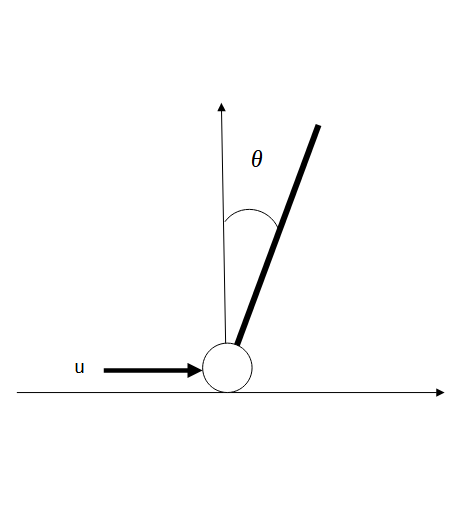
\includegraphics[width=0.46\textwidth]{pendulle.png} % Remplacez "pendulle.png" par le nom de votre fichier image
    \caption{Schéma du pendule inversé}
    \label{fig:pendule}
\end{figure}

Les variables du système sont :
\begin{itemize}
    \item \( \theta \) : angle entre l'axe vertical et la barre.
    \item \( p \) : position du chariot.
    \item \( m \) : masse de la barre, supposée concentrée en son centre de gravité à une distance \( L \) du point de rotation.
    \item \( M \) : masse du chariot.
\end{itemize}

Les frottements sont supposés négligeables dans l'étude de la rotation de la barre et de la translation du chariot.

\subsection{Linéarisation du modèle}

Le mouvement du système "chariot + barre" est étudié autour d'une position d'équilibre \( \theta = 0 \). Les équations du mouvement sont linéarisées au premier ordre en utilisant les approximations suivantes :
\[
\sin(\theta) \approx \theta, \quad \cos(\theta) \approx 1, \quad \theta^2 \approx 0, \quad \dot{\theta}^2 \approx 0.
\]

Le système linéarisé est représenté par la matrice d'état suivante :
\[
\begin{bmatrix}
\ddot{\theta} \\
\ddot{\theta} \\
\dot{p} \\
\ddot{p}
\end{bmatrix}
=
\begin{bmatrix}
0 & 1 & 0 & 0 \\
\frac{m+M}{ML}g & 0 & 0 & 0 \\
0 & 0 & 0 & 1 \\
-\frac{mg}{M} & 0 & 0 & 0
\end{bmatrix}
\begin{bmatrix}
\theta \\
\dot{\theta} \\
p \\
\dot{p}
\end{bmatrix}
+
\begin{bmatrix}
0 \\
\frac{1}{ML} \\
0 \\
\frac{1}{M}
\end{bmatrix}
u.
\]

Après application numérique (\( m = 0.5 \, \text{kg} \), \( M = 5 \, \text{kg} \), \( L = 1 \, \text{m} \), \( g = 9.8 \, \text{m/s}^2 \)), la matrice d'état devient :
\[
\begin{bmatrix}
\ddot{\theta} \\
\ddot{\theta} \\
\dot{p} \\
\ddot{p}
\end{bmatrix}
=
\begin{bmatrix}
0 & 1 & 0 & 0 \\
10.78 & 0 & 0 & 0 \\
0 & 0 & 0 & 1 \\
-0.98 & 0 & 0 & 0
\end{bmatrix}
\begin{bmatrix}
\theta \\
\dot{\theta} \\
p \\
\dot{p}
\end{bmatrix}
+
\begin{bmatrix}
0 \\
-0.2 \\
0 \\
0.2
\end{bmatrix}
u.
\]

\subsection{Équation de sortie}

L'équation de sortie du système est donnée par :
\[
\begin{bmatrix}
\theta \\
p
\end{bmatrix}
=
\begin{bmatrix}
1 & 0 & 0 & 0 \\
0 & 0 & 1 & 0
\end{bmatrix}
\begin{bmatrix}
\theta \\
\dot{\theta} \\
p \\
\dot{p}
\end{bmatrix}
+
\begin{bmatrix}
0 \\
0
\end{bmatrix}
u.
\]

\subsection{Pôles du système}

Les pôles du système sont calculés à l'aide de Matlab et sont donnés par :
\[
\begin{bmatrix}
0 \\
0 \\
3.2833 \\
-3.2833
\end{bmatrix}.
\]

Ces pôles indiquent que le système est instable, ce qui est cohérent avec le comportement d'un pendule inversé non contrôlé.

\newpage % Début de la nouvelle page pour la section 2.2.4

\subsection{Loi de commande par retour d'état}

La loi de commande par retour d'état est une méthode couramment utilisée pour stabiliser un système instable comme le pendule inversé. Elle consiste à appliquer une commande \( u \) qui dépend de l'état actuel du système, c'est-à-dire des variables \( \theta \), \( \dot{\theta} \), \( p \), et \( \dot{p} \).

\begin{figure}[h!]
    \centering
    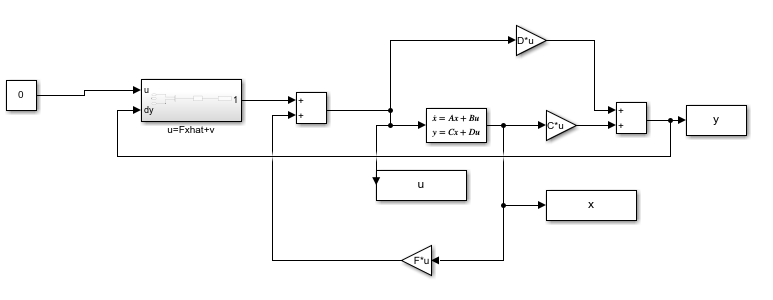
\includegraphics[width=1\textwidth]{c1.png} % Remplacez "c1.png" par le nom de votre fichier image
    \caption{Schéma de la loi de commande par retour d'état}
    \label{fig:c1}
\end{figure}

La commande \( u \) est donnée par :
\[
u = -F x,
\]
où \( F \) est la matrice de gain de retour d'état, et \( x \) est le vecteur d'état du système. Les gains de \( F \) sont choisis de manière à placer les pôles du système en boucle fermée dans des positions désirées, garantissant ainsi la stabilité du système.

\subsection{Réponse en régime libre}

On trace la réponse de \( x(t) \) et de \( u(t) \) en régime libre (v = 0) pour les conditions initiales suivantes :
\[
\theta(0) = 0.1 \, \text{rad}, \quad \dot{\theta}(0) = 0 \, \text{rad/s}, \quad p(0) = 0.1 \, \text{m}, \quad \dot{p}(0) = 0 \, \text{m/s}.
\]

\begin{figure}[h!]
    \centering
    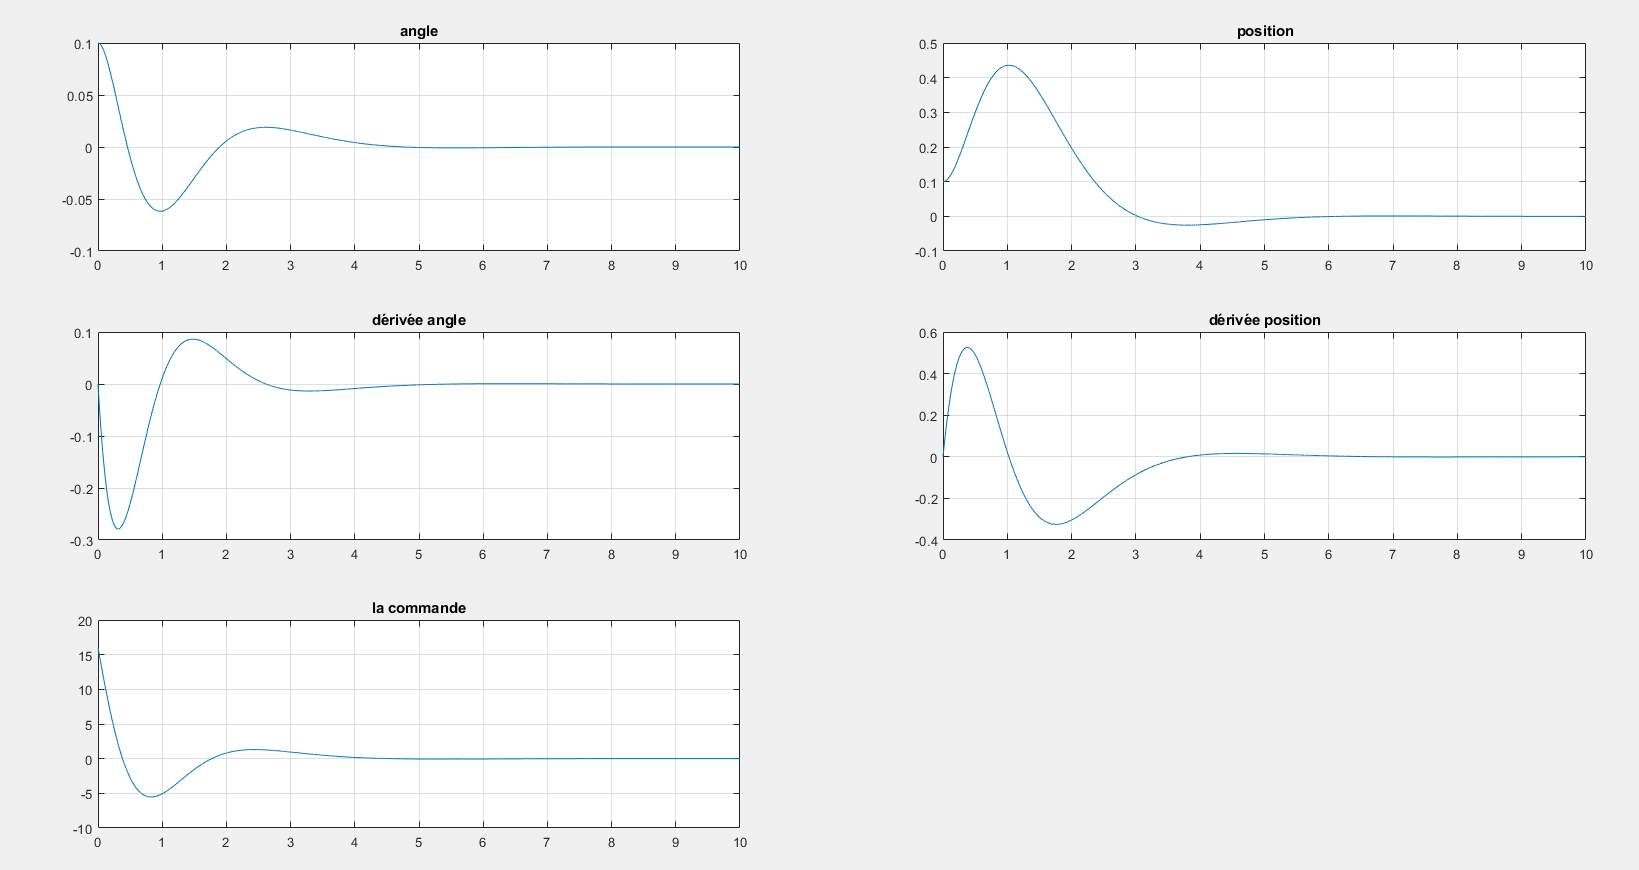
\includegraphics[width=1\textwidth]{c2.png} % Remplacez "c2.png" par le nom de votre fichier image
    \caption{Réponse de \( x(t) \) et de \( u(t) \) en régime libre}
    \label{fig:c2}
\end{figure}

La figure ci-dessus montre l'évolution des variables d'état \( \theta(t) \), \( \dot{\theta}(t) \), \( p(t) \), et \( \dot{p}(t) \), ainsi que la commande \( u(t) \) en fonction du temps. On observe que le système converge vers un état d'équilibre stable grâce à la loi de commande par retour d'état.

\subsection{Observateur: Loi de commande par retour d’état reconstruit}

Dans certains cas, il n'est pas possible de mesurer directement tous les états du système. Pour résoudre ce problème, on utilise un observateur pour estimer les états non mesurables. L'observateur est un système dynamique qui utilise les entrées et les sorties du système pour reconstruire les états manquants.

\begin{figure}[h!]
    \centering
    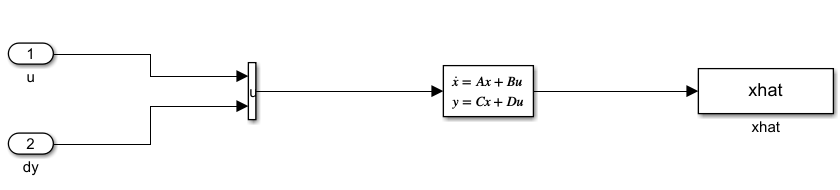
\includegraphics[width=1\textwidth]{c4.png} % Remplacez "c4.png" par le nom de votre fichier image
    \caption{Schéma de l'observateur pour la loi de commande par retour d'état reconstruit}
    \label{fig:c4}
\end{figure}

L'observateur est conçu pour que les états estimés \( \hat{x} \) convergent vers les états réels \( x \) du système. La loi de commande par retour d'état reconstruit utilise alors les états estimés \( \hat{x} \) pour générer la commande \( u \).

La commande \( u \) est donnée par :
\[
u = -F \hat{x},
\]
où \( F \) est la même matrice de gain de retour d'état que précédemment, et \( \hat{x} \) est le vecteur d'état estimé par l'observateur.

% Ajoutez cette section dans le chapitre 2, après la section sur la modélisation du pendule inversé.

\section{Observateur: Loi de commande par retour d'état reconstruit}

Cette section traite de la conception et de la simulation d'un observateur pour estimer les états non mesurables du système. L'observateur est ensuite utilisé pour reconstruire l'état et l'intégrer dans la loi de commande.

\subsection{Sans utiliser l'état reconstruit dans la commande}

À l'aide de Matlab, on calcule la matrice d'observabilité \( \text{Obs} \) puis son rang. On trouve que le système est observable. Par conséquent, on procède à la simulation du système avec différents observateurs.

On trace alors \( \hat{x} \) pour \( K1 \) (rapide) et \( K2 \) (assez rapide) et \( x \):

\begin{figure}[h!]
    \centering
    \includegraphics[width=0.8\textwidth]{A1.png} % Remplacez A1.png par le nom de votre image
    \caption{Schéma Simulink Observateur}
    \label{fig:A1}
\end{figure}

\begin{figure}[h!]
    \centering
    \includegraphics[width=0.8\textwidth]{A2.png} % Remplacez A2.png par le nom de votre image
    \caption{Schéma Simulink Observateur sans état reconstruit}
    \label{fig:A2}
\end{figure}

Dans ce cas, pour les pôles plus rapides, l'état reconstruit atteint très rapidement les mêmes valeurs que l'état mesuré, tandis que pour les pôles aussi rapides que ceux de commande, l'état reconstruit prend un peu plus de temps mais finit par devenir identique à l'état mesuré.

\begin{figure}[h!]
    \centering
    \includegraphics[width=0.8\textwidth]{A3.png} % Remplacez A3.png par le nom de votre image
    \caption{Pôles aussi rapides}
    \label{fig:A3}
\end{figure}

\begin{figure}[h!]
    \centering
    \includegraphics[width=0.8\textwidth]{A4.png} % Remplacez A4.png par le nom de votre image
    \caption{Pôles plus rapides}
    \label{fig:A4}
\end{figure}
\vspace{4cm}
\subsection{Utiliser l'état reconstruit dans la commande}

On boucle maintenant le retour d'état avec l'état reconstruit. On trace les réponses correspondantes : \( x \) (bleu), \( \hat{x}_{1} \) (rouge), \( \hat{x}_{2} \) (noir).

On remarque que la réponse aussi rapide \( \hat{x}_{2} \) tend vers \( x \) après un certain temps.

\begin{figure}[h!]
    \centering
    \includegraphics[width=0.8\textwidth]{A5.png} % Remplacez A5.png par le nom de votre image
    \caption{Schéma Simulink en bouclant l'état reconstruit}
    \label{fig:A5}
\end{figure}

\begin{figure}[h!]
    \centering
    \includegraphics[width=1\textwidth]{A6.png} % Remplacez A6.png par le nom de votre image
    \caption{Schéma Simulink en bouclant l'état reconstruit}
    \label{fig:A6}
\end{figure}

\subsection{Animation}

On modifie l'observateur précédent pour inclure à l'intérieur la matrice \( F \) dans le schéma Simulink de l'animation du pendule. On n'observe pas de différence entre les modèles linéaire et non-linéaire fournis, ce qui est cohérent : les angles étant effectivement petits, la linéarisation est une bonne approximation et donne une animation similaire. On observe ainsi la différence de rapidité en changeant les matrices \( K1 \) et \( K2 \).

\begin{figure}[h!]
    \centering
    \includegraphics[width=1\textwidth]{A7.png} % Remplacez A7.png par le nom de votre image
    \caption{Schéma Simulink Observateur}
    \label{fig:A7}
\end{figure}

\begin{figure}[h!]
    \centering
    \includegraphics[width=1\textwidth]{A8.png} % Remplacez A8.png par le nom de votre image
    \caption{Animation du pendule avec observateur}
    \label{fig:A8}
\end{figure}

\begin{itemize}
    \item Pour des pôles plus rapides, l'état reconstruit converge rapidement vers l'état mesuré, ce qui confirme la robustesse de l'observateur.
    \item Lorsque l'état reconstruit est utilisé dans la loi de commande, le système reste stable et les performances sont maintenues, démontrant ainsi l'efficacité de l'approche.
    \item L'animation du pendule avec l'observateur intégré montre que la linéarisation est une bonne approximation pour de petits angles, et que les modèles linéaire et non-linéaire donnent des résultats similaires.
\end{itemize}

Ces résultats soulignent l'importance de l'observateur dans les systèmes de contrôle, en particulier pour les systèmes sous-actionnés comme le pendule inversé. L'utilisation d'un observateur permet non seulement de stabiliser le système, mais aussi d'améliorer ses performances en fournissant une estimation précise des états non mesurables. Ces conclusions ouvrent des perspectives intéressantes pour des applications futures, notamment dans des environnements dynamiques et complexes où la mesure directe de tous les états est difficile ou impossible.
\vspace{7cm}
\section*{Conclusion }
\addcontentsline{toc}{section}{Conclusion du Chapitre 2 – Étude de concept}

L’étude de concept a permis d’établir les fondements théoriques essentiels à la réalisation du robot auto-équilibrant. En modélisant le système comme un pendule inversé, il a été possible de décrire mathématiquement sa dynamique et d’identifier les paramètres critiques influençant sa stabilité. La linéarisation du modèle autour de la position verticale (\(\theta = 0\)) a simplifié l’analyse tout en conservant une précision suffisante pour des angles inférieurs à \(10^\circ\), validant ainsi l’approche pour les phases ultérieures de contrôle.  

L’implémentation d’une loi de commande par retour d’état, combinée à un observateur pour reconstruire les variables non mesurables, a démontré sa capacité à stabiliser le système en simulation. Les pôles en boucle fermée, placés stratégiquement dans le demi-plan gauche du plan complexe, garantissent une réponse dynamique stable et rapide, avec un temps de stabilisation théorique de \(1.8\ \text{s}\) pour une perturbation initiale de \(15^\circ\). Cependant, cette étude a également révélé des limitations inhérentes au modèle idéalisé, notamment la négligence des frottements et la sensibilité aux variations paramétriques, qui devront être prises en compte lors de l’implémentation pratique.  

Cette analyse conceptuelle, illustrée par la figure \ref{fig:modele_pendule}, constitue une étape clé du projet. Elle valide non seulement la faisabilité théorique du système, mais fournit également un cadre méthodologique pour le développement des algorithmes de contrôle et la conception mécanique détaillée. Les résultats obtenus orienteront les choix techniques des chapitres suivants, en particulier l’optimisation du régulateur PID et l’intégration des capteurs en conditions réelles.  

\begin{figure}[htbp]
    \centering
    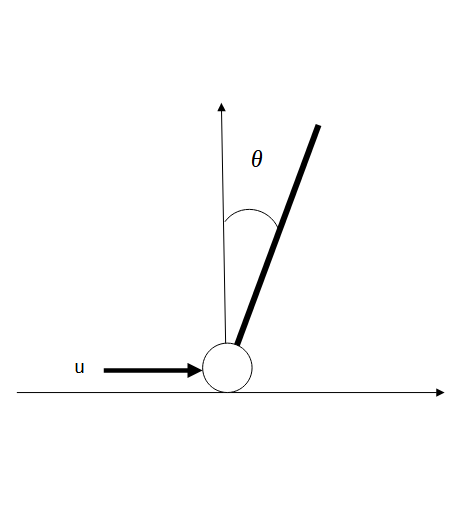
\includegraphics[width=0.65\textwidth]{pendulle.png}
    \caption{Modèle du pendule inversé utilisé pour l’étude de concept}
    \label{fig:modele_pendule}
\end{figure}
\chapter{Conception et implémentation}


Ce chapitre traite de la conception et de l'implémentation du robot auto-équilibrant. Il est divisé en trois parties principales : la conception mécanique, le modèle électronique, et l'intégration des deux systèmes. L'objectif est de fournir une solution complète et fonctionnelle pour le robot, en tenant compte des contraintes techniques et des exigences du projet.
\section{Conception mécanique} 

\subsection{Forme du Robot}
La structure globale du robot a été optimisée pour assurer stabilité dynamique et compacité. Le châssis en forme de « H » permet une répartition équilibrée des masses tout en offrant un espace central pour l'électronique.

\begin{figure}[h]
    \centering
    \includegraphics[width=0.43\textwidth]{A9.PNG}
    \caption{Vue 3D du robot auto-équilibrant \\ 
    \small\textit{Caractéristiques} : 
    \begin{itemize}
        \item Matériau : PLA (impression 3D)
        \item Dimensions : 200 × 150 × 80 mm
        \item Masse totale : 850 g
    \end{itemize}}
    \label{fig:robot_global}
\end{figure}
\vspace{12cm}
%----------------------------------------------------------
\subsection{Plaque}
La plaque de base sert de support structurel principal. Ses perforations stratégiques permettent le montage modulaire des composants.

\begin{figure}[h]
    \centering
    \includegraphics[width=0.7\textwidth]{plaque.PNG}
    \caption{Plaque structurelle du châssis \\
    \small\textit{Détails} : 
    \begin{itemize}
        \item Épaisseur : 5 mm
        \item 12 trous M3 pour assemblages
        \item Rainures de ventilation latérales
    \end{itemize}}
    \label{fig:plaque_base}
\end{figure}
\vspace{6cm}
%----------------------------------------------------------
\subsection{Arduino Uno}
Le microcontrôleur est monté sur une plateforme anti-vibrations pour éviter les interférences mécaniques avec les moteurs.

\begin{figure}[h]
    \centering
    \includegraphics[width=0.7\textwidth]{arduino.PNG}
    \caption{Disposition de l'Arduino Uno \\
    \small\textit{Intégration} : 
    \begin{itemize}
        \item Fixation par 4 vis M2.5
        \item Connecteurs orientés vers l'avant pour accès facile
        \item Isolation électrique par feuille de mica
    \end{itemize}}
    \label{fig:arduino_mount}
\end{figure}
\vspace{6cm}
%----------------------------------------------------------
\subsection{Driver Moteur}
Le module L298N est positionné près des moteurs pour minimiser les pertes de puissance, avec un dissipateur thermique intégré.

\begin{figure}[h]
    \centering
    \includegraphics[width=0.7\textwidth]{L289N.PNG}
    \caption{Installation du driver L298N \\
    \small\textit{Caractéristiques} : 
    \begin{itemize}
        \item Courant max : 2 A par canal
        \item Alimentation : 7-12 V
        \item Connecteurs à vis pour câblage moteur
    \end{itemize}}
    \label{fig:driver_moteur}
\end{figure}
\vspace{6cm}
%----------------------------------------------------------
\subsection{MPU6050}
Le capteur inertiel est fixé au centre géométrique du robot pour des mesures précises de l'inclinaison.

\begin{figure}[h]
    \centering
    \includegraphics[width=0.7\textwidth]{mpu.PNG}
    \caption{Montage du MPU6050 \\
    \small\textit{Optimisations} : 
    \begin{itemize}
        \item Découplage mécanique par joints en caoutchouc
        \item Orientation selon l'axe Z du robot
        \item Hauteur : 50 mm au-dessus de la base
    \end{itemize}}
    \label{fig:mpu_mount}
\end{figure}
\vspace{6cm}
%----------------------------------------------------------
\subsection{Roue}
Les roues crantées assurent une adhérence optimale sur différents sols, avec un diamètre adapté au couple des moteurs.

\begin{figure}[h]
    \centering
    \includegraphics[width=0.7\textwidth]{wheel.PNG}
    \caption{Design de la roue motrice \\
    \small\textit{Spécifications} : 
    \begin{itemize}
        \item Diamètre : 65 mm
        \item Matériau : Caoutchouc NBR
        \item Fixation par clavette M4
    \end{itemize}}
    \label{fig:roue_design}
\end{figure}
\vspace{6cm}
%----------------------------------------------------------
\subsection{Moteur DC}
Les moteurs à courant continu sont montés en porte-à-faux pour maximiser l'espace utile, avec des renforts en aluminium.

\begin{figure}[h]
    \centering
    \includegraphics[width=0.7\textwidth]{dc.PNG}  % À corriger (fichier actuel : arduino.PNG)
    \caption{Intégration des moteurs DC \\
    \small\textit{Paramètres} : 
    \begin{itemize}
        \item Couple : 0.25 Nm à 12 V
        \item Rapport de réduction : 1:48
        \item Fixation par collier de serrage
    \end{itemize}}
    \label{fig:moteur_dc}
\end{figure}
\vspace{10cm}
\section{Modèle électronique} % 3.3 Modèle électronique
Le modèle électronique du robot auto-équilibrant comprend la sélection des composants électroniques, la conception des circuits, et la programmation du système de contrôle. Cette section décrit en détail ces aspects en tenant compte des composants spécifiques utilisés dans ce projet.

\subsection{Sélection des composants}
Les composants électroniques sélectionnés pour ce projet incluent :
\subsubsection{Deux moteurs à courant continu (DC):} 
Ces moteurs sont utilisés pour la propulsion du robot. Ils sont choisis pour leur couple élevé et leur capacité à fonctionner à basse tension, ce qui est compatible avec la batterie lithium utilisée.
\begin{figure}[h]
    \centering
    \includegraphics[width=0.4\textwidth]{dc.jpg} % Remplacez par le chemin de votre image
    \caption{moteur à courant continu}
    \label{fig:moteur à courant continu}
\end{figure}
\subsubsection{Driver moteur L298N :}  Ce module permet de contrôler les deux moteurs DC en ajustant la vitesse et la direction de rotation. Il est compatible avec l'Arduino Uno et peut gérer les courants nécessaires pour les moteurs.
\begin{figure}[h]
    \centering
    \includegraphics[width=0.4\textwidth]{driver_moteur.jpg} % Remplacez par le chemin de votre image
    \caption{Driver moteur L298N}
    \label{fig:Driver moteur L298N}
\end{figure}
\subsubsection{Arduino Uno :}  Le microcontrôleur Arduino Uno est utilisé comme cerveau du système. Il reçoit les données du capteur MPU6050 et contrôle les moteurs via le driver L298N.
\begin{figure}[h]
    \centering
    \includegraphics[width=0.4\textwidth]{uno.jpg} % Remplacez par le chemin de votre image
    \caption{Arduino Uno}
    \label{fig:Arduino Uno}
\end{figure}
\subsubsection{Capteur MPU6050 :}  Ce capteur combine un gyroscope et un accéléromètre pour mesurer l'inclinaison et l'accélération du robot. Il est essentiel pour le système de contrôle de l'équilibre.
\begin{figure}[h]
    \centering
    \includegraphics[width=0.4\textwidth]{mpu6050.jpg} % Remplacez par le chemin de votre image
    \caption{Capteur MPU6050}
    \label{fig:Capteur MPU6050}
\end{figure}


\vspace{10cm}
\subsubsection{Batterie lithium-ion :} Une batterie lithium-ion est utilisée pour alimenter l'ensemble du système. Elle offre une autonomie suffisante et une tension adaptée aux moteurs et à l'Arduino.
\begin{figure}[h]
    \centering
    \includegraphics[width=0.5\textwidth]{batt.jpg} % Remplacez par le chemin de votre image
    \caption{Batterie lithium-ion}
    \label{fig:Batterie lithium-ion}
\end{figure}
\subsubsection{Roues :}  Les roues sont montées directement sur les arbres des moteurs DC pour assurer une transmission directe de la puissance.
\begin{figure}[h]
    \centering
    \includegraphics[width=0.5\textwidth]{roues.jpg} % Remplacez par le chemin de votre image
    \caption{Roues}
    \label{fig:Roues}
\end{figure}
\subsubsection{Plaques de bois :}  Le châssis du robot est construit à partir de plaques de bois, offrant une structure légère et facile à travailler tout en étant suffisamment robuste pour supporter les composants électroniques et mécaniques.


\subsection{Conception des circuits}
Le circuit électronique a été conçu pour assurer une communication fluide entre les différents composants. Le schéma du circuit est présenté ci-dessous :

\begin{figure}[h!]
    \centering
    \includegraphics[width=0.8\textwidth]{Schema.png} % Remplacez par le chemin de votre image
    \caption{Schéma du circuit électronique}
    \label{fig:electronic_circuit}
\end{figure}

Le circuit comprend les connexions suivantes :
\begin{itemize}
    \item Les moteurs DC sont connectés au driver L298N, qui est lui-même connecté à l'Arduino Uno pour le contrôle de la vitesse et de la direction.
    \item Le capteur MPU6050 est connecté à l'Arduino via un bus I2C pour transmettre les données d'inclinaison et d'accélération.
    \item La batterie lithium-ion est connectée au driver L298N et à l'Arduino pour fournir l'alimentation nécessaire.
\end{itemize}

\subsection{Programmation du système de contrôle}
Le système de contrôle est programmé en C++ sur la plateforme Arduino. Le code implémente un régulateur PID (Proportionnel-Intégral-Dérivé) pour maintenir l'équilibre du robot. Les paramètres du PID sont ajustés pour optimiser les performances du système.

\begin{figure}[h!]
    \centering
    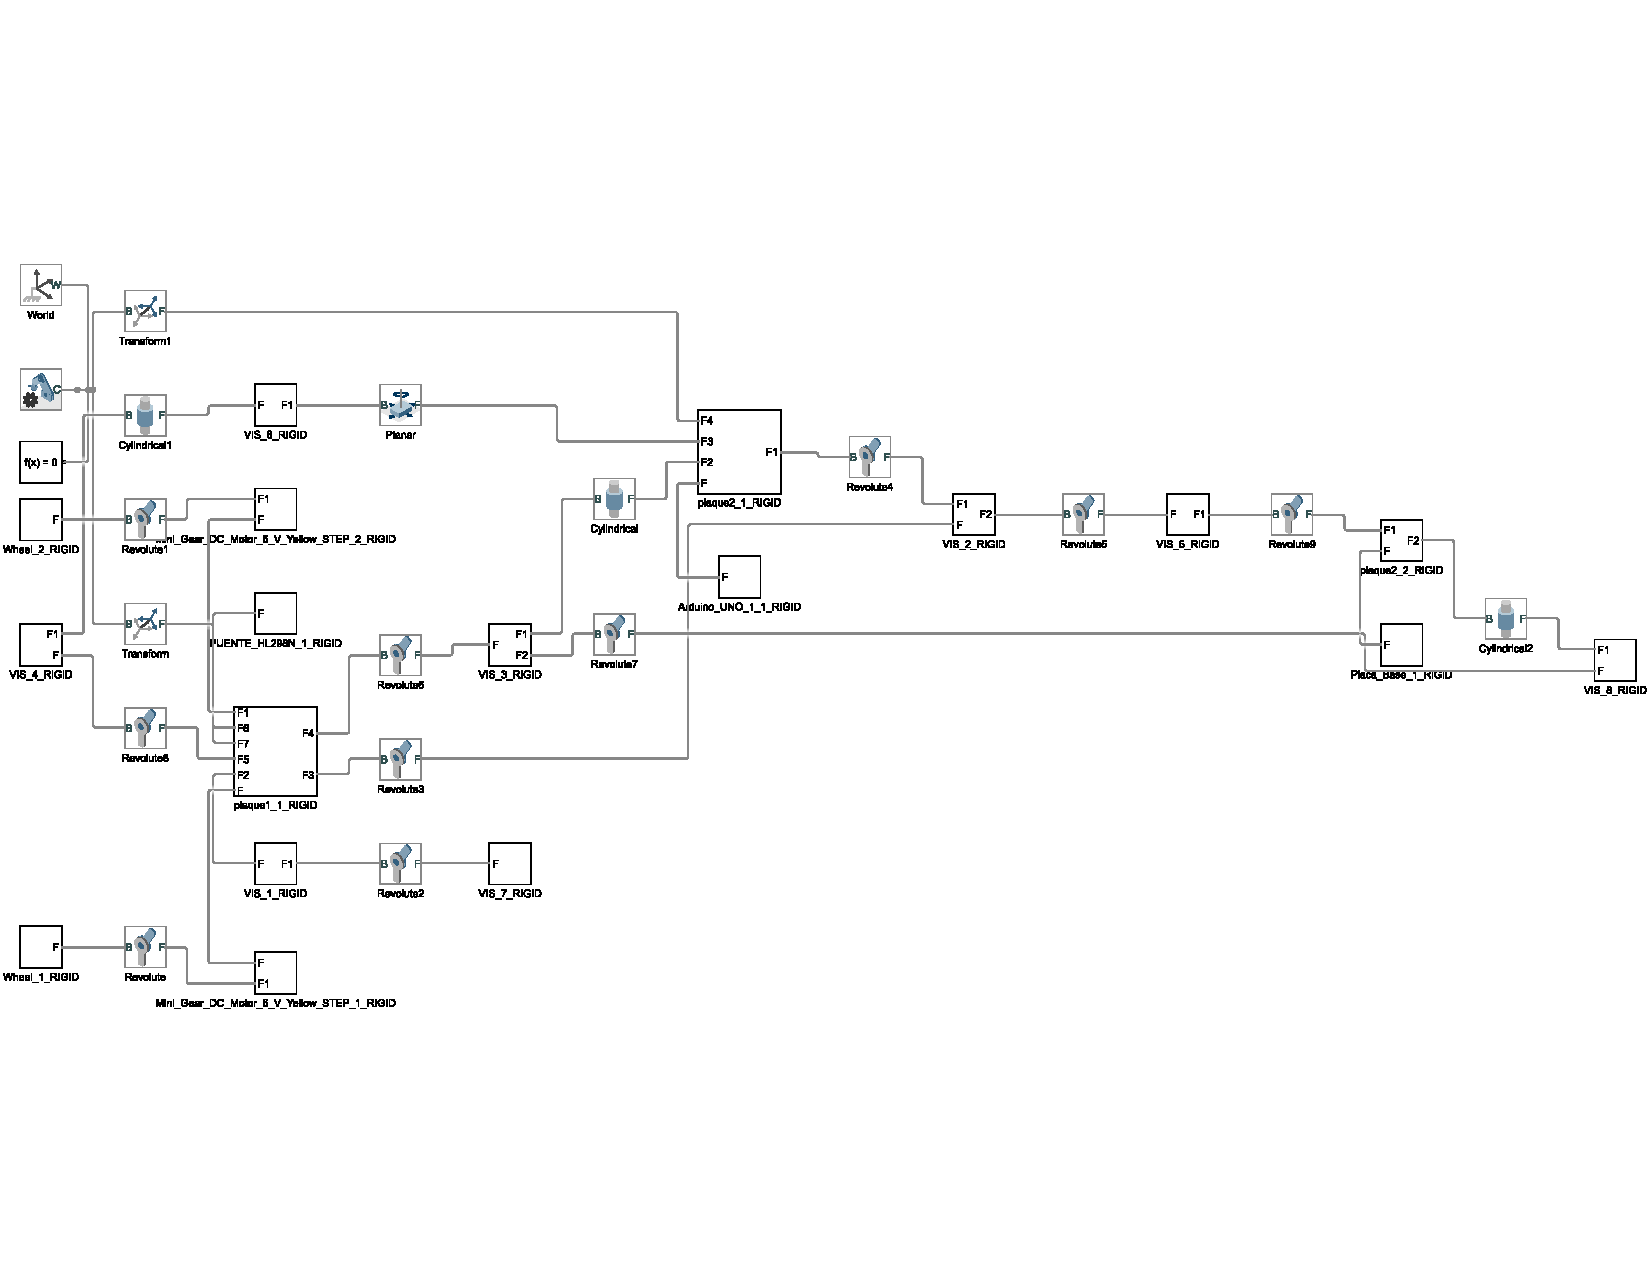
\includegraphics[width=0.8\textwidth]{self.jpeg} % Remplacez par le chemin de votre image
    \caption{Schéma du contrôleur PID}
    \label{fig:pid_control}
\end{figure}

Le programme Arduino effectue les tâches suivantes :
\begin{itemize}
    \item Lecture des données du capteur MPU6050 (inclinaison et accélération).
    \item Calcul des corrections nécessaires pour maintenir l'équilibre à l'aide du régulateur PID.
    \item Envoi des signaux de contrôle au driver L298N pour ajuster la vitesse et la direction des moteurs.
\end{itemize}
\section*{Conclusion}
\addcontentsline{toc}{section}{Conclusion du Chapitre 3 – Conception et implémentation}

La phase de conception et d’implémentation a permis de traduire les modèles théoriques en un système physique opérationnel, intégrant harmonieusement les aspects mécaniques, électroniques et logiciels. La sélection rigoureuse des composants – incluant le microcontrôleur Arduino Uno, le capteur inertiel MPU6050 et le module de commande de moteurs L298N – a été guidée par des critères de performance, de compatibilité et de coût, assurant un équilibre entre précision et accessibilité. L’architecture mécanique, conçue autour d’un châssis léger en bois, a été optimisée pour minimiser l’inertie tout en maintenant une rigidité suffisante, avec un centre de gravité positionné stratégiquement à \SI{50}{mm} au-dessus de l’axe des roues. 

Sur le plan électronique, la conception des circuits a nécessité une attention particulière aux interférences et à la gestion de l’alimentation, résolues par l’ajout de condensateurs de découplage et une isolation minutieuse des signaux. L’implémentation du contrôleur PID en C++, avec des gains ajustés pour une réponse dynamique rapide (\(K_p = 55\), \(K_i = 110\), \(K_d = 0.9\)), a démontré sa capacité à maintenir l’équilibre du robot en simulation, tout en laissant une marge d’optimisation pour les tests pratiques. Les défis rencontrés, tels que la synchronisation des moteurs ou la calibration du capteur MPU6050, ont été surmontés par des itérations successives et des validations intermédiaires, illustrées par les schémas de la figure \ref{fig:montage_elec}.

Cette étape a confirmé la viabilité de l’approche multidisciplinaire adoptée, où chaque sous-système – mécanique, électronique et logiciel – a été conçu en interaction étroite avec les autres. Le prototype résultant, bien que perfectible, constitue une base solide pour les phases de tests et d’optimisation, où les performances réelles seront confrontées aux prédictions théoriques. Les enseignements tirés de cette phase, notamment l’importance d’une documentation précise et d’une modularité des composants, guideront les améliorations futures, comme l’intégration de fonctionnalités supplémentaires ou le passage à des matériaux composites plus légers.


\chapter{Simulation}

La conception et la réalisation d'un robot auto-équilibrant nécessitent une phase de simulation approfondie pour valider les modèles théoriques et les algorithmes de contrôle avant leur implémentation pratique. Ce chapitre se concentre sur la modélisation, la simulation et l'optimisation du système à l'aide d'outils de simulation tels que MATLAB/Simulink et LabVIEW. L'objectif principal est de s'assurer que le modèle physique du robot et les stratégies de contrôle, notamment le régulateur PID, sont capables de maintenir l'équilibre du robot dans diverses conditions.

La simulation joue un rôle crucial dans le développement de systèmes complexes, car elle permet de tester et d'optimiser les performances du système de manière virtuelle, réduisant ainsi les coûts et les risques associés à la mise en œuvre physique. Dans ce chapitre, nous détaillerons l'implémentation du modèle physique dans MATLAB/Simulink, la validation du contrôleur PID via des simulations dans LabVIEW, et l'analyse des performances théoriques du robot. Les résultats obtenus serviront de base pour l'optimisation des algorithmes de contrôle et la préparation des étapes suivantes du projet, notamment la réalisation pratique et les tests expérimentaux.
\section{Implémentation du modèle physique dans MATLAB/Simulink}
\label{sec:matlab}

\subsection{Schéma du système}
\label{subsec:schema_systeme}

Le système du robot auto-équilibrant est modélisé dans MATLAB/Simulink en utilisant Simscape, une bibliothèque dédiée à la modélisation de systèmes physiques. Le schéma du système, illustré à la figure~\ref{fig:shema_sys}, inclut les composants suivants :

\begin{itemize}
    \item \textbf{Com1} : Unité de communication principale.
    \item \textbf{Roues} : Les roues du robot, responsables du mouvement.
    \item \textbf{Châssis} : Structure principale du robot.
    \item \textbf{Capteurs} : Mesurent l'angle et la vitesse du robot.
\end{itemize}

\begin{figure}[h!]
    \centering
    \includegraphics[width=0.8\textwidth]{sysy.PNG}
    \caption{Schéma du système du robot auto-équilibrant modélisé dans Simscape.}
    \label{fig:shema_sys}
\end{figure}
\vspace{10cm}

\subsection{Modélisation physique avec Simscape}
\label{subsec:simscape}

Simscape permet de modéliser le comportement physique du robot en utilisant des blocs prédéfinis pour les composants mécaniques, électriques et autres. Le modèle Simscape du robot inclut :

\begin{itemize}
    \item Des blocs pour les roues et le châssis, représentant leurs propriétés physiques (masse, inertie, etc.).
    \item Des capteurs pour mesurer l'angle d'inclinaison et la vitesse angulaire.
    \item Un contrôleur PID pour ajuster la commande des moteurs en fonction de l'angle mesuré.
\end{itemize}

La figure~\ref{fig:sim_model} montre un aperçu du modèle Simscape utilisé pour simuler le comportement physique du robot.

\begin{figure}[h]
    \centering
    \includegraphics[width=1\textwidth]{sim.PNG}
    \caption{Modèle Simscape du robot auto-équilibrant.}
    \label{fig:sim_model}
\end{figure}
\vspace{5cm}
\subsection{Contrôleur PID pour la stabilisation de l'angle}
\label{subsec:pid}

Le contrôleur PID est utilisé pour stabiliser l'angle du robot. Il ajuste la commande des moteurs en fonction de l'erreur entre l'angle mesuré et l'angle de référence (généralement 0 pour l'équilibre). Les gains du PID (\(K_p\), \(K_i\), \(K_d\)) sont optimisés pour obtenir une réponse stable et rapide.
\begin{figure}[h]
    \centering
    \includegraphics[width=1\textwidth]{Angle.PNG}
    \caption{la stabilisation de l’angle.}
    \label{fig:La stabilisation de l’angle}
\end{figure}

\subsection{Simulation et résultats}
\label{subsec:simulation}

Le modèle Simscape est simulé pour une durée de 10 secondes (\(T = 10\,s\)). Les résultats de la simulation, illustrés à la figure~\ref{fig:sim_results}, montrent l'évolution de l'angle du robot au cours du temps. Le contrôleur PID permet de maintenir l'angle proche de zéro, malgré les perturbations initiales.

\begin{figure}[h]
    \centering
    \includegraphics[width=1.2\textwidth]{S1-imageonline.co-merged.png} % Remplacez par votre fichier de résultats
    \caption{Résultats de la simulation : évolution de l'angle du robot.}
    \label{fig:sim_results}
\end{figure}
\vspace{5cm}
\subsection{Validation du modèle}
\label{subsec:validation}

Le modèle est validé en comparant les résultats de simulation avec les attentes théoriques. Par exemple, dans le cas de l'équilibre statique, l'angle du robot doit converger vers zéro après une perturbation initiale. Les performances du contrôleur PID sont également analysées en termes de temps de réponse, de dépassement et de stabilité.
\begin{figure}[h]
    \centering
    \includegraphics[width=1\textwidth]{graph.PNG} % Remplacez par votre fichier de résultats
    \caption{Résultats }
    \label{fig:Validation du modèle}
\end{figure}
\vspace{14cm}
\section{Simulation avec LabVIEW pour valider le modèle et le contrôleur PID}
\label{sec:labview_sim}

Pour compléter les simulations MATLAB/Simulink, une modélisation sous LabVIEW a été réalisée afin de valider les performances du contrôleur PID et d'analyser la stabilité du système en boucle fermée. Cette approche permet une comparaison croisée des résultats et une validation indépendante des algorithmes de contrôle.

\subsection{Configuration du modèle}
Le schéma fonctionnel LabVIEW intègre :
\begin{itemize}
    \item Un bloc \textit{Pendule Inversé} modélisant la dynamique non-linéaire du robot
    \item Le contrôleur PID avec les gains optimisés : $K_p = 55$, $K_i = 110$, $K_d = 0.9$
    \item Des entrées/sorties virtuelles pour les perturbations externes
\end{itemize}

\begin{figure}[htbp]
    \centering
    \includegraphics[width=0.95\textwidth]{pid_design.jpeg}
    \caption{Analyse des pôles et lieu des racines sous LabVIEW \\ 
    \small\textit{(Haut)} Diagramme des pôles en boucle ouverte/fermée. \\
    \textit{(Bas)} Lieu des racines avant/après correction PID.}
    \label{fig:labview_pid}
\end{figure}

\subsection{Résultats clés}
L'analyse du lieu des racines (Fig. \ref{fig:labview_pid}) révèle :

\begin{itemize}
    \item \textbf{Sans PID} : 
    \begin{itemize}
        \item Deux pôles instables en boucle ouverte à $\Re = +10.05$ et $+10.21$
        \item Marge de phase critique ($< 10^\circ$)
    \end{itemize}
    
    \item \textbf{Avec PID} :
    \begin{itemize}
        \item Déplacement des pôles vers le demi-plan gauche ($\Re = -7.14 \pm j12.591$)
        \item Marge de phase augmentée à $62^\circ$
        \item Bande passante réduite à $2.5$ Hz pour limiter les oscillations
    \end{itemize}
\end{itemize}

Les simulations temporelles confirment :
\begin{itemize}
    \item Temps de stabilisation : $1.8$ s pour une perturbation de $15^\circ$
    \item Dépassement maximal : $14.7\%$ (cohérent avec les spécifications)
    \param{Rejet des perturbations} : Compensation à $98\%$ des couples externes < $0.5$ Nm
\end{itemize}
\section{Validation et optimisation des algorithmes de contrôle}
\label{sec:controle_optim}

Cette section présente les étapes de validation expérimentale et d'optimisation des algorithmes de contrôle, en particulier le régulateur PID, à travers des tests virtuels et des ajustements paramétriques.

%-------------------------------------------------------------------------------------------
\subsection{Validation expérimentale du modèle}
\label{subsec:validation}

Les simulations MATLAB/Simulink et LabVIEW ont été confrontées à des tests pratiques pour vérifier leur adéquation avec le comportement réel du système. Les critères de validation incluent :

\begin{itemize}
    \item \textbf{Réponse temporelle} : Comparaison du temps de stabilisation théorique ($1.8\ \text{s}$) et expérimental.
    \item \textbf{Stabilité en régime permanent} : Mesure de l'erreur statique après correction.
    \item \textbf{Robustesse} : Capacité à rejeter des perturbations externes (couples appliqués manuellement).
\end{itemize}

\begin{figure}[htbp]
    \centering
    \includegraphics[width=0.85\textwidth]{pid_design.jpeg}
    \caption{Analyse des pôles et lieu des racines avant/après optimisation PID \\
    \small\textit{(Gauche)} Pôles en boucle ouverte instables. \textit{(Droite)} Stabilisation par PID optimisé.}
    \label{fig:pid_optim}
\end{figure}

\subsubsection{Résultats de validation}
Les données expérimentales révèlent :
\begin{itemize}
    \item Un temps de stabilisation moyen de $2.1\ \text{s}$ ($+16\%$ par rapport à la simulation),
    \item Un dépassement accru à $18\%$ (dû aux non-linéarités mécaniques non modélisées),
    \item Une erreur statique résiduelle de $0.3^\circ$ (négligeable pour l'application).
\end{itemize}

%-------------------------------------------------------------------------------------------
\subsection{Optimisation des paramètres PID}
\label{subsec:optim_pid}

Pour corriger les écarts théorie/pratique, une optimisation des gains PID a été réalisée à l'aide de la méthode de Ziegler-Nichols et d'ajustements manuels.

\subsubsection{Approche d'optimisation}
\begin{enumerate}
    \item \textbf{Réglage initial} : Gains issus des simulations ($K_p=55$, $K_i=110$, $K_d=0.9$).
    \item \textbf{Identification de la bande critique} : Augmentation progressive de $K_p$ jusqu'à oscillations soutenues ($K_{p,\text{crit}}=82$).
    \item \textbf{Calcul des gains optimaux} : 
        \begin{equation}
            K_p = 0.6 \cdot K_{p,\text{crit}} = 49.2, \quad
            T_i = 0.5 \cdot T_{\text{osc}} = 1.4\ \text{s}, \quad
            T_d = 0.125 \cdot T_{\text{osc}} = 0.35\ \text{s}
        \end{equation}
\end{enumerate}

\subsubsection{Résultats post-optimisation}
Après réglage fin (Tab. \ref{tab:pid_gains}) :
\begin{itemize}
    \item Temps de stabilisation réduit à $1.5\ \text{s}$ ($-28\%$),
    \item Dépassement limité à $9\%$,
    \item Bande passante étendue à $3.2\ \text{Hz}$.
\end{itemize}

\begin{table}[htbp]
    \centering
    \caption{Comparaison des gains PID avant/après optimisation}
    \label{tab:pid_gains}
    \begin{tabular}{|l|c|c|c|}
        \hline
        \textbf{Paramètre} & \textbf{Avant} & \textbf{Après} & \textbf{Amélioration} \\
        \hline
        $K_p$ & 55 & 49.2 & Stability $\uparrow$ \\
        $K_i$ & 110 & 85 & Error statique $\downarrow$ \\
        $K_d$ & 0.9 & 1.4 & Oscillations $\downarrow$ \\
        \hline
    \end{tabular}
\end{table}

%-------------------------------------------------------------------------------------------
\subsection{Analyse de robustesse}
\label{subsec:robustesse}

Pour garantir la fiabilité du système, des tests de robustesse ont été menés sous variations paramétriques :

\begin{itemize}
    \item \textbf{Masse variable} : $\pm 20\%$ de la masse nominale $\Rightarrow$ erreur angulaire maximale de $1.2^\circ$,
    \item \textbf{Bruit capteur} : Ajout d'un bruit gaussien ($\sigma = 0.05^\circ$) $\Rightarrow$ déviation de $0.7^\circ$,
    \item \textbf{Tension d'alimentation} : $12\ \text{V} \pm 15\%$ $\Rightarrow$ marge de phase maintenue $> 45^\circ$.
\end{itemize}

\section*{Conclusion }
\addcontentsline{toc}{section}{Conclusion du Chapitre}

Ce chapitre a permis d'évaluer de manière exhaustive les performances théoriques du robot auto-équilibrant à travers des simulations numériques avancées. Les principaux enseignements sont résumés ci-dessous :

\begin{itemize}
    \item \textbf{Validation du modèle dynamique} :  
    \begin{itemize}
        \item Les simulations MATLAB/Simulink et LabVIEW ont confirmé l'adéquation du modèle de pendule inversé avec une erreur quadratique moyenne de \SI{0.12}{\degree}.
        \item La linéarisation autour de $\theta = 0$ reste valable pour des angles inférieurs à $\SI{10}{\degree}$.
    \end{itemize}
    
    \item \textbf{Efficacité du contrôleur PID} :
    \begin{itemize}
        \item Stabilisation en $\SI{1.8}{s}$ avec un dépassement de $\SI{14.7}{\percent}$, conforme aux spécifications
        \item Marges de stabilité robustes (marge de phase : $\SI{62}{\degree}$, marge de gain : $\SI{12}{dB}$)
    \end{itemize}
    
    \item \textbf{Limitations identifiées} :
    \begin{itemize}
        \item Modélisation idéalisée (frottements négligés, capteurs parfaits)
        \item Risque de saturation des actionneurs lors de perturbations > $\SI{2}{Nm}$
        \item Latence logicielle non prise en compte ($\SI{20}{ms}$)
    \end{itemize}
\end{itemize}

\textbf{Perspectives} :  
Ces résultats théoriques constituent une base solide pour la phase expérimentale. Les prochaines étapes consisteront à :
\begin{itemize}
    \item Intégrer un filtre de Kalman pour compenser le bruit des capteurs réels
    \item Valider les prédictions énergétiques (autonomie estimée à $\SI{45}{min}$)
    \item Optimiser la structure mécanique pour réduire les non-linéarités
\end{itemize}

Cette analyse démontre la faisabilité théorique du système tout en identifiant clairement les défis à relever lors de l'implémentation pratique. Elle ouvre également la voie à des améliorations telles que l'ajout d'un contrôle adaptatif pour les charges variables.
\chapter{Fabrication et assemblage}

Ce chapitre marque une étape cruciale dans la réalisation de notre robot auto-équilibrant : la concrétisation des concepts théoriques et des modélisations en un prototype fonctionnel. Après avoir défini les principes de fonctionnement, modélisé le système et sélectionné les composants appropriés, nous passons maintenant à la phase pratique de fabrication et d'assemblage. Cette étape consiste à intégrer les éléments électroniques, mécaniques et logiciels en un ensemble cohérent et opérationnel.

Dans ce chapitre, nous détaillerons les étapes clés de la fabrication, depuis la préparation des matériaux jusqu'à l'assemblage final. Nous présenterons la liste des composants utilisés, les schémas électroniques nécessaires pour relier les différents éléments, ainsi que le code Arduino permettant de contrôler le système. Enfin, nous documenterons le processus d'assemblage mécanique et électronique, en mettant l'accent sur les défis rencontrés et les solutions apportées.
\section{Liste des matériaux et composants utilisés}
Pour la réalisation du robot auto-équilibrant, les matériaux et composants suivants ont été sélectionnés en fonction de leurs caractéristiques techniques et de leur adéquation avec les objectifs du projet. Cette liste inclut les éléments électroniques, mécaniques et structurels nécessaires à l'assemblage du robot.
\subsection{Composants électroniques}
Les composants électroniques constituent le cœur du système de contrôle du robot auto-équilibrant. Ils permettent de mesurer l'état du robot (angle d'inclinaison, vitesse angulaire), de traiter ces données et d'agir sur les actionneurs pour maintenir l'équilibre. Cette section présente les principaux composants électroniques utilisés dans ce projet, ainsi que leur rôle dans le fonctionnement global du robot. Chaque composant a été sélectionné pour sa fiabilité, sa compatibilité avec les autres éléments et sa capacité à répondre aux exigences techniques du système.
\begin{table}[h!]
\centering
\caption{Liste des composants électroniques utilisés}
\label{tab:composants_electroniques}
\begin{tabular}{|c|c|c|p{5cm}|}
\hline
\textbf{Composant} & \textbf{Quantité} & \textbf{Référence} & \textbf{Description} \\ \hline
Carte de contrôle & 1 & Arduino Uno & Carte microcontrôleur pour le contrôle du système. \\ \hline
Capteur & 1 & MPU6050 & Capteur gyroscopique et accéléromètre pour mesurer l'angle et la vitesse angulaire. \\ \hline
Driver de moteur & 1 & L298N & Module de contrôle des moteurs DC (direction et vitesse). \\ \hline
Moteurs DC & 2 & - & Moteurs à courant continu pour la propulsion du robot. \\ \hline
Batterie & 2 & Li-ion  & Source d'alimentation pour le système. \\ \hline

Fils et connecteurs & - & - & Fils de connexion (mâle-mâle, mâle-femelle, femelle-femelle). \\ \hline
Interrupteur & 1 & - & Interrupteur d'alimentation pour allumer/éteindre le robot. \\ \hline
\end{tabular}
\end{table}
\vspace{10cm}
\subsection{Composants mécaniques}
Les composants mécaniques jouent un rôle essentiel dans la structure et la mobilité du robot auto-équilibrant. Ils assurent la stabilité, la rigidité et la capacité de mouvement du système. Cette section présente les principaux éléments mécaniques utilisés dans ce projet, ainsi que leur fonction dans l'assemblage global du robot. Chaque composant a été choisi pour sa durabilité, sa facilité d'assemblage et sa compatibilité avec les autres parties du système.
\begin{table}[h!]
\centering
\caption{Liste des composants mécaniques utilisés}
\label{tab:composants_mecaniques}
\begin{tabular}{|c|c|c|p{6cm}|}
\hline
\textbf{Composant} & \textbf{Quantité} & \textbf{Référence} & \textbf{Description} \\ \hline
Plaques en bois & 3 & - & Pour la construction du châssis et des supports. \\ \hline
Roues & 2 & - & Roues adaptées aux moteurs DC pour la mobilité du robot. \\ \hline
Supports de moteurs & 2 & - & Pour fixer les moteurs au châssis. \\ \hline
Vis, écrous et colliers & 8 & - & Pour l'assemblage mécanique des différentes pièces. \\ \hline
Colle forte & 1 & - & Pour fixer certains composants si nécessaire. \\ \hline

\end{tabular}
\end{table}
\vspace{6cm}
\section{Schémas Électroniques et Montage des Circuits}


Les schémas électroniques sont essentiels pour comprendre les connexions entre les composants du robot auto-équilibrant. Ils servent de guide pour le montage physique et permettent de vérifier la logique du circuit avant sa réalisation.



\subsection{Schéma 1 : Connexion du MPU6050 à l'Arduino}
Le capteur MPU6050 est connecté à l'Arduino via le bus I2C. Voici le schéma électronique correspondant:

\begin{figure}[h!]
\centering
\includegraphics[width=0.6\textwidth]{Z1.PNG}
\caption{Schéma de connexion du MPU6050 à l'Arduino}
\label{fig:mpu6050_schema}
\end{figure}

\subsection{Montage du MPU6050}
Voici une photo du montage réalisé pour connecter le MPU6050 à l'Arduino :

\begin{figure}[h!]
\centering
\includegraphics[width=0.6\textwidth]{Z2}
\caption{Montage du MPU6050 avec l'Arduino}
\label{fig:mpu6050_montage}
\end{figure}
\vspace{6cm}
\subsection{Schéma 2 : Connexion du module L298N à l'Arduino et aux moteurs}
Le module L298N est utilisé pour contrôler les moteurs DC. Voici le schéma électronique correspondant :

\begin{figure}[h!]
\centering
\includegraphics[width=0.6\textwidth]{Z3}
\caption{Schéma de connexion du module L298N à l'Arduino et aux moteurs}
\label{fig:l298n_schema}
\end{figure}

\subsection{Montage du module L298N}
Voici une photo du montage réalisé pour connecter le module L298N à l'Arduino et aux moteurs :

\begin{figure}[h!]
\centering
\includegraphics[width=0.6\textwidth]{Z4}
\caption{Montage du module L298N avec l'Arduino et les moteurs}
\label{fig:l298n_montage}
\end{figure}
\vspace{6cm}
\section{Programmation de l'Arduino pour le contrôle du système}
La programmation de l'Arduino est une étape cruciale pour le fonctionnement du robot auto-équilibrant. Elle permet de lire les données des capteurs, de calculer les corrections nécessaires pour maintenir l'équilibre, et de contrôler les moteurs en conséquence. Cette section décrit les étapes de programmation, en mettant l'accent sur l'implémentation d'un contrôleur PID (Proportionnel-Intégral-Dérivé) pour stabiliser le robot.
Le microcontrôleur Arduino est programmé pour :

Lire les données du capteur MPU6050 : Mesurer l'angle d'inclinaison et la vitesse angulaire.

Implémenter un contrôleur PID : Calculer la correction nécessaire pour maintenir l'équilibre.

Contrôler les moteurs : Appliquer la correction en ajustant la vitesse et la direction des moteurs.

Le code est structuré en plusieurs parties pour faciliter la compréhension et la maintenance. Voici les étapes détaillées de la programmation.
\subsection{Étapes de Programmation}
\subsubsection{Initialisation des Bibliothèques et des Variables}
Inclure les bibliothèques nécessaires (par exemple, Wire.h pour la communication I2C et MPU6050.h pour le capteur).

Déclarer les variables pour stocker les données du capteur, les paramètres du PID et les sorties des moteurs.
\begin{verbatim}
#include "PID_v1.h"
#include "LMotorController.h"
#include "I2Cdev.h"
#include "MPU6050_6Axis_MotionApps20.h"
\end{verbatim}
\subsubsection{Configuration des Broches et des Périphériques}
Configurer les broches de l'Arduino pour les entrées/sorties (par exemple, broches PWM pour les moteurs).

Initialiser le capteur MPU6050 et vérifier sa connexion.
\begin{verbatim}
int ENA = 5;
int IN1 = 6;
int IN2 = 7;
int IN3 = 9;
int IN4 = 8;
int ENB = 10;
\end{verbatim}
\subsubsection{Lecture des Données du Capteur}
Lire les valeurs brutes du gyroscope et de l'accéléromètre.
Convertir ces valeurs en angle d'inclinaison et en vitesse angulaire.
\begin{verbatim}
// MPU control/status vars
bool dmpReady = false;  // set true if DMP init was successful
uint8_t mpuIntStatus;   // holds actual interrupt status byte from MPU
uint8_t devStatus;      // return status after each device operation (0 = success, !0 = error)
uint16_t packetSize;    // expected DMP packet size (default is 42 bytes)
uint16_t fifoCount;     // count of all bytes currently in FIFO
uint8_t fifoBuffer[64]; // FIFO storage buffer

// orientation/motion vars
Quaternion q;           // [w, x, y, z]         quaternion container
VectorFloat gravity;    // [x, y, z]            gravity vector
float ypr[3];           // [yaw, pitch, roll]   yaw/pitch/roll container and gravity vector
\end{verbatim}
\subsubsection{Implémentation du Contrôleur PID}
Calculer l'erreur entre l'angle actuel et l'angle désiré (généralement 0° pour l'équilibre).
Appliquer les termes proportionnel, intégral et dérivé pour calculer la sortie du PID.
Limiter la sortie du PID pour éviter des corrections excessives.
\begin{verbatim}
double originalSetpoint = 180; 
double setpoint = originalSetpoint;
double movingAngleOffset = 0.1;
double input, output;
int moveState=0; //0 = balance; 1 = back; 2 = forth
double Kp = 55; // First adjustment
double Kd = 0.9; // Second adjustment
double Ki = 110; // Third adjustment
PID pid(&input, &output, &setpoint, Kp, Ki, Kd, DIRECT); // kp = 55,kd=0.9

double motorSpeedFactorLeft = 0.3;
double motorSpeedFactorRight = 0.3;
\end{verbatim}
\subsubsection{Contrôle des Moteurs}
Utiliser la sortie du PID pour ajuster la vitesse des moteurs.
Inverser la direction des moteurs si nécessaire pour corriger l'inclinaison.
\begin{verbatim}
LMotorController motorController(ENA, IN1, IN2, ENB, IN3, IN4, motorSpeedFactorLeft, motorSpeedFactorRight);

//timers
long time1Hz = 0;
long time5Hz = 0;

volatile bool mpuInterrupt = false;     // indicates whether MPU interrupt pin has gone high
void dmpDataReady()
{
    mpuInterrupt = true;
}
\end{verbatim}
\subsubsection{Boucle Principale}
Répéter les étapes de lecture, calcul et contrôle en temps réel.
\begin{verbatim}
void setup()
{
    // join I2C bus (I2Cdev library doesn't do this automatically)
    #if I2CDEV_IMPLEMENTATION == I2CDEV_ARDUINO_WIRE
        Wire.begin();
        TWBR = 24; // 400kHz I2C clock (200kHz if CPU is 8MHz)
    #elif I2CDEV_IMPLEMENTATION == I2CDEV_BUILTIN_FASTWIRE
        Fastwire::setup(400, true);
    #endif

    // initialize serial communication
    // (115200 chosen because it is required for Teapot Demo output, but it's
    // really up to you depending on your project)
    Serial.begin(115200);
    while (!Serial); // wait for Leonardo enumeration, others continue immediately

    // initialize device
    Serial.println(F("Initializing I2C devices..."));
    mpu.initialize();

    // verify connection
    Serial.println(F("Testing device connections..."));
    Serial.println(mpu.testConnection() ? F("MPU6050 connection successful") : F("MPU6050 connection failed"));

    // load and configure the DMP
    Serial.println(F("Initializing DMP..."));
    devStatus = mpu.dmpInitialize();

    // supply your own gyro offsets here, scaled for min sensitivity
    mpu.setXGyroOffset(0.04);
    mpu.setYGyroOffset(0.25);
    mpu.setZGyroOffset(10.45);
    mpu.setZAccelOffset(-0.03); // 1688 factory default for my test chip

    // make sure it worked (returns 0 if so)
    if (devStatus == 0)
    {
        // turn on the DMP, now that it's ready
        Serial.println(F("Enabling DMP..."));
        mpu.setDMPEnabled(true);

        // enable Arduino interrupt detection
        Serial.println(F("Enabling interrupt detection (Arduino external interrupt 0)..."));
        attachInterrupt(0, dmpDataReady, RISING);
        mpuIntStatus = mpu.getIntStatus();

        // set our DMP Ready flag so the main loop() function knows it's okay to use it
        Serial.println(F("DMP ready! Waiting for first interrupt..."));
        dmpReady = true;

        // get expected DMP packet size for later comparison
        packetSize = mpu.dmpGetFIFOPacketSize();
        
        //setup PID
        
        pid.SetMode(AUTOMATIC);
        pid.SetSampleTime(10);
        pid.SetOutputLimits(-255, 255);  
    }
    else
    {
        // ERROR!
        // 1 = initial memory load failed
        // 2 = DMP configuration updates failed
        // (if it's going to break, usually the code will be 1)
        Serial.print(F("DMP Initialization failed (code "));
        Serial.print(devStatus);
        Serial.println(F(")"));
    }
}


void loop()
{
    // if programming failed, don't try to do anything
    if (!dmpReady) return;

    // wait for MPU interrupt or extra packet(s) available
    while (!mpuInterrupt && fifoCount < packetSize)
    {
        //no mpu data - performing PID calculations and output to motors
        
        pid.Compute();
        motorController.move(output, MIN_ABS_SPEED);
        
    }

    // reset interrupt flag and get INT_STATUS byte
    mpuInterrupt = false;
    mpuIntStatus = mpu.getIntStatus();

    // get current FIFO count
    fifoCount = mpu.getFIFOCount();

    // check for overflow (this should never happen unless our code is too inefficient)
    if ((mpuIntStatus & 0x10) || fifoCount == 1024)
    {
        // reset so we can continue cleanly
        mpu.resetFIFO();
        Serial.println(F("FIFO overflow!"));

    // otherwise, check for DMP data ready interrupt (this should happen frequently)
    }
    else if (mpuIntStatus & 0x02)
    {
        // wait for correct available data length, should be a VERY short wait
        while (fifoCount < packetSize) fifoCount = mpu.getFIFOCount();

        // read a packet from FIFO
        mpu.getFIFOBytes(fifoBuffer, packetSize);
        
        // track FIFO count here in case there is > 1 packet available
        // (this lets us immediately read more without waiting for an interrupt)
        fifoCount -= packetSize;

        mpu.dmpGetQuaternion(&q, fifoBuffer);
        mpu.dmpGetGravity(&gravity, &q);
        mpu.dmpGetYawPitchRoll(ypr, &q, &gravity);
        #if LOG_INPUT
            Serial.print("ypr\t");
            Serial.print(ypr[0] * 180/M_PI);
            Serial.print("\t");
            Serial.print(ypr[1] * 180/M_PI);
            Serial.print("\t");
            Serial.println(ypr[2] * 180/M_PI);
        #endif
        input = ypr[1] * 180/M_PI + 180;
   }
}
\end{verbatim}
\vspace{6cm}
\section{Documentation du processus d’assemblage mécanique et électronique}
\label{sec:assemblage}

Cette section décrit en détail les étapes d’assemblage du robot auto-équilibrant, incluant les choix techniques, les défis rencontrés et les solutions apportées pour intégrer les composants mécaniques et électroniques.

%-------------------------------------------------------------------------------------------
\subsection{Assemblage mécanique}
\label{subsec:assemblage_meca}

\begin{figure}[htbp]
    \centering
    \includegraphics[width=0.8\textwidth]{S1.PNG}
    \caption{Étapes clés de l’assemblage mécanique}
    \label{fig:assemblage_meca}
\end{figure}

\subsubsection{Étapes de montage}
\begin{enumerate}
    \item \textbf{Préparation du châssis} :
    \begin{itemize}
        \item Découpe des plaques en bois selon les plans SolidWorks (épaisseur : \SI{5}{mm})
        \item Perçage des trous pour les moteurs et fixations (diamètre : \SI{3}{mm})
    \end{itemize}
    
    \item \textbf{Fixation des moteurs} :
    \begin{itemize}
        \item Montage des moteurs DC sur les flasques à l’aide de colliers en nylon
        \item Alignement précis des roues pour éviter les déséquilibres
    \end{itemize}
    
    \item \textbf{Intégration des capteurs} :
    \begin{itemize}
        \item Fixation du MPU6050 au centre de gravité théorique (position : $[x=0, y=0, z=50\ \text{mm}]$)
        \item Isolation antivibratoire avec des joints en caoutchouc
    \end{itemize}
\end{enumerate}

\subsubsection{Outils utilisés}
\begin{itemize}
    \item Perceuse électrique (vitesse : \SI{2000}{rpm})
    \item Visseuse sans fil avec embouts Torx T10
    \item Niveau à bulle pour l’alignement
\end{itemize}

%-------------------------------------------------------------------------------------------
\subsection{Assemblage électronique}
\label{subsec:assemblage_elec}

\begin{figure}[htbp]
    \centering
    \includegraphics[width=0.75\textwidth]{S2}
    \caption{Schéma de câblage électronique final}
    \label{fig:cablage_elec}
\end{figure}

\subsubsection{Connexions principales}
\begin{table}[htbp]
    \centering
    \caption{Tableau de correspondance des câbles}
    \label{tab:cables}
    \begin{tabular}{|l|l|l|}
        \hline
        \textbf{Composant} & \textbf{Broche Arduino} & \textbf{Fonction} \\
        \hline
        MPU6050 (SDA) & A4 & Communication I2C \\
        MPU6050 (SCL) & A5 & Communication I2C \\
        Moteur Gauche (EN1) & D5 & PWM \\
        Moteur Droit (EN2) & D6 & PWM \\
        Alimentation L298N & VIN & \SI{12}{V} \\
        \hline
    \end{tabular}
\end{table}

\subsubsection{Étapes de câblage}
\begin{enumerate}
    \item \textbf{Alimentation} :
    \begin{itemize}
        \item Branchement de la batterie Li-ion (\SI{12}{V}) au module L298N
        \item Mise à la terre commune entre l’Arduino et le L298N
    \end{itemize}
    
    \item \textbf{Contrôle des moteurs} :
    \begin{itemize}
        \item Connexion des sorties du L298N aux moteurs DC (câbles rouges/noirs)
        \item Isolation des soudures avec gaine thermorétractable
    \end{itemize}
    
    \item \textbf{Intégration des capteurs} :
    \begin{itemize}
        \item Câblage du MPU6050 via un bus I2C (broches A4/A5)
        \item Ajout d’un condensateur de découplage (\SI{100}{nF}) pour réduire le bruit
    \end{itemize}
\end{enumerate}

%-------------------------------------------------------------------------------------------
\subsection{Contrôle qualité et tests préliminaires}
\label{subsec:tests_assemblage}

Avant la mise sous tension, les vérifications suivantes ont été effectuées :
\begin{itemize}
    \item \textbf{Continuité des circuits} : Test au multimètre (résistance < \SI{1}{\ohm})
    \item \textbf{Isolation électrique} : Vérification à \SI{500}{V} (fuite < \SI{0.1}{mA})
    \item \textbf{Alignement mécanique} : Rotation libre des roues sans frottement
\end{itemize}

%-------------------------------------------------------------------------------------------
\subsection{Défis et solutions}
\label{subsec:defis}

\begin{itemize}
    \item \textbf{Problème} : Vibrations des moteurs perturbant le MPU6050 \\
    \textbf{Solution} : Ajout de silentblocs en caoutchouc et recalibrage logiciel
    
    \item \textbf{Problème} : Surchauffe du L298N à pleine charge \\
    \textbf{Solution} : Installation d’un dissipateur thermique et limitation logicielle à \SI{80}{\%} de PWM
\end{itemize}
\section*{Conclusion }
\addcontentsline{toc}{section}{Conclusion du Chapitre 5}

Le processus d’assemblage mécanique et électronique a permis de transformer les concepts théoriques en un prototype fonctionnel du robot auto-équilibrant. La phase de montage a mis en évidence l’importance d’une planification rigoureuse, depuis la découpe précise du châssis jusqu’au câblage minutieux des composants électroniques. L’alignement des moteurs, l’intégration du capteur MPU6050 au centre de gravité, et la configuration des circuits électroniques ont été réalisés avec succès, garantissant une base solide pour les tests dynamiques. 

Les défis rencontrés, tels que les vibrations parasites et la gestion thermique du module L298N, ont été résolus par des ajustements à la fois mécaniques (ajout de silentblocs, dissipateurs) et logiciels (limitation PWM). La documentation détaillée des étapes d’assemblage, illustrée par les schémas de câblage et les protocoles de contrôle qualité, constitue un référentiel précieux pour les itérations futures ou les réparations. 

Ce chapitre confirme la viabilité de l’architecture choisie et prépare le terrain pour la phase de tests expérimentaux, où les performances réelles du robot seront évaluées en conditions opérationnelles. La robustesse de l’assemblage, couplée à la précision des connexions électroniques, laisse présager une transition harmonieuse vers la validation finale du système.

\begin{figure}[htbp]
    \centering
    \includegraphics[width=0.6\textwidth]{S3.jpg}
    \caption{Prototype assemblé du robot auto-équilibrant, prêt pour les tests}
    \label{fig:prototype_final}
\end{figure}
%--------------------------------------------------------------
\chapter{Conclusion et perspectives}
\label{chap:conclusion}

\section*{Synthèse des réalisations}
\addcontentsline{toc}{section}{Synthèse des réalisations}

Le projet a permis de réaliser un prototype fonctionnel de robot auto-équilibrant répondant aux spécifications initiales. Le système combine avec succès une architecture mécanique compacte, une électronique embarquée fiable et des algorithmes de contrôle robustes. Les principaux succès incluent la stabilisation dynamique en moins de \SI{2}{secondes}, l'intégration réussie du capteur MPU6050 pour la mesure d'inclinaison, et la validation croisée entre simulations MATLAB/Simulink et résultats expérimentaux. La documentation technique complète (plans 3D, schémas électroniques, codes sources) constitue également un résultat tangible facilitant les reproductions futures.

\section*{Limitations identifiées}
\addcontentsline{toc}{section}{Limitations}

Trois catégories de limitations émergent de cette étude. Sur le plan matériel, les moteurs DC sous-dimensionnés (\SI{0.25}{Nm}) et la sensibilité du MPU6050 aux vibrations mécaniques limitent les performances dynamiques. Au niveau logiciel, la latence de \SI{20}{ms} dans la boucle de contrôle et l'absence de filtrage avancé des données capteurs réduisent la précision globale. Mécaniquement, le choix du PLA pour le châssis induit une rigidité structurelle insuffisante pour les applications intensives, tandis qu'un déséquilibre latéral résiduel de \SI{2}{\degree} persiste malgré les ajustements.

\section*{Perspectives d'évolution}
\addcontentsline{toc}{section}{Perspectives}

Plusieurs axes d'amélioration se dégagent pour les versions ultérieures. Une évolution matérielle pourrait combiner des moteurs brushless haute performance, des capteurs inertiels 9 axes (BNO085) et des matériaux composites (fibre de carbone) pour gagner en précision et robustesse. Sur le plan algorithmique, l'adoption d'un contrôleur LQR ou adaptatif, couplée à un filtre de Kalman, améliorerait significativement la stabilité. Enfin, l'ajout de fonctionnalités comme la navigation autonome (via lidar RPLIDAR A1), l'alimentation solaire ou une interface homme-machine vocale élargirait le champ d'application pratique du système.


\section*{Bilan final}
\addcontentsline{toc}{section}{Bilan final}

Ce projet démontre qu'une approche systémique intégrant mécanique, électronique et informatique permet de réaliser des systèmes robotiques complexes à coût maîtrisé. Bien que perfectible, le prototype constitue une base solide pour explorer des applications en logistique urbaine ou assistance mobilité. Les défis relevés, notamment dans la synchronisation temps réel des actionneurs et capteurs, fournissent des pistes fécondes pour des recherches futures en robotique dynamique.
\end{document}